\subsection{Attention moves within an identical wrist image}
\label{sec:supp-spatial-attention}
Does attention to the wrist image change when only the main view changes? In one fixed example it does, at L9 and L18 while L1 stays near zero, although the wrist pixels are identical (Fig.~\ref{fig:attention-spatial-full}). This is an additional illustration for the attention analysis; the main paper does not rely on it. The signed row shows where conditional attention rises or falls on average; the magnitude row keeps changes that cancel in the signed average.

\begin{figure*}[t]
\centering
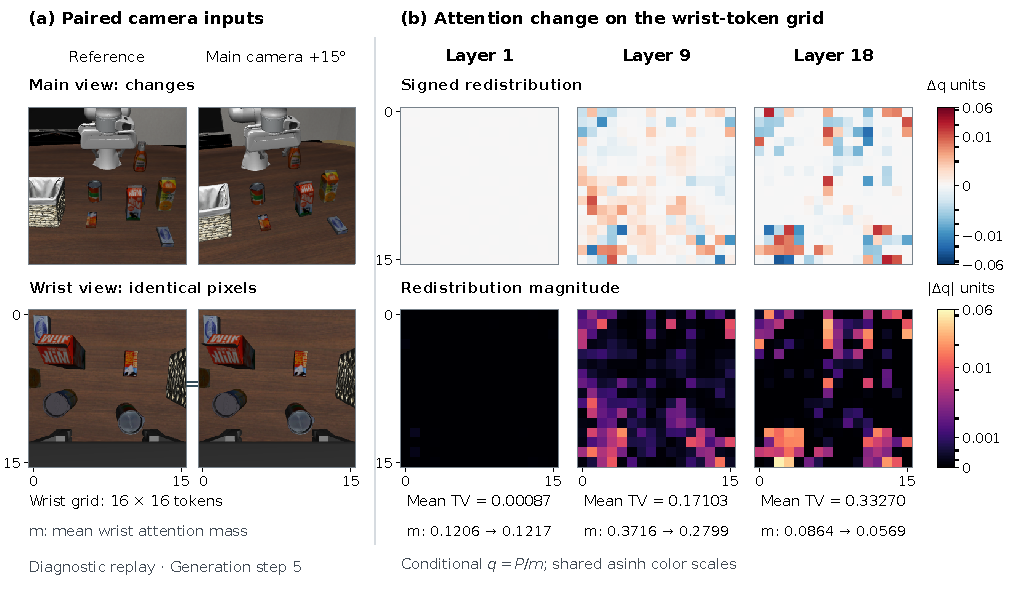
\includegraphics[width=\textwidth]{figures/attention_spatial_full.pdf}
\caption{\textbf{Conditional attention redistributes over identical wrist pixels.} (a) The physical state and instruction are fixed. Main-camera yaw changes from $0^\circ$ to $15^\circ$ at the baseline headlight setting; the wrist images are pixel-identical. (b) Conditional attention at generation step $j=5$, with matched state, time and noise. For each of eight heads and ten plan positions, $q_k=P_k/m$, where $m=\sum_{k\in\mathrm{wrist}}P_k$, and $\Delta q=q_{\rm changed}-q_{\rm reference}$. Rows show $\langle\Delta q\rangle$ and $\langle|\Delta q|\rangle$ over all 80 head--position entries (eight heads $\times$ ten plan positions) in this one fixed example, taking absolute values before averaging in the second row. Each row shares one asinh color scale across layers, with ticks in probability units. Mean TV is $\langle\tfrac12\sum_k|\Delta q_k|\rangle$; mass values read reference $\rightarrow$ changed. The top-left image origin and token coordinates are shared by all panels.}
\label{fig:attention-spatial-full}
\end{figure*}

\paragraph{One fixed example, all heads and positions.}
The example is the first, in lexicographic order, of an existing eight-state gallery from the fixed-state camera study: LIBERO-10 task 01, demonstration 7, early frame 1, with the instruction ``put both the cream cheese box and the butter in the basket.'' All of L1/L9/L18 and every head--position pair are shown, without selection by response size or outcome. Raw wrist pixels and the wrist inputs the policy consumes are verified identical, and the main-camera inputs differ. The example uses the common-noise record at $j=5$; Table~\ref{tab:legacy-attention} reports the separate $j=0$ comparison over 36 tasks.

\paragraph{Reading direction, magnitude and mass together.}
The magnitude map averages $|\Delta q|$ at each token before display, and the mean TV below each layer sums absolute changes before averaging, whereas the signed map allows cancellation across heads and positions. The regional mass $m$ places each conditional distribution within attention over all keys. L1 stays near zero on the shared scale, while L9 and L18 show spatial redistribution. All three layers use one scale, symmetric about zero for the signed row and starting at zero for the magnitude row; no values are clipped or rescaled by layer. A rounding-interval check at L1 is compatible for all 80 head--position entries; it is a compatibility check, not a measured bound on numerical error.

\paragraph{Spatial addresses.}
Each map is a $16\times16$ grid in the policy's image orientation: local index $k=16y+x$ maps to wrist prefix key $256+k$, with $x$ increasing rightward and $y$ downward. The original $256\times256$ RGB image and the consumed $224\times224$ image cover the same square field; each model patch is $14\times14$ consumed pixels. The maps keep this orientation without flip, rotation or crop. They show conditional probabilities from a replay of the saved attention.

\paragraph{Implementation notes.}
The color scale has asinh linear width $0.0009429195779375732$ and absolute limit $0.060346852988004684$, taken from the original gallery.
